\documentclass[13pt ,a4paper ]{report}

\usepackage[utf8]{inputenc}
\usepackage[T1]{fontenc}      % caractères français
\usepackage[francais]{babel}  %langue
\usepackage[left=2.3cm,right=2.5cm,bottom=2.5cm,top=2.3cm]{geometry}   % marges
\usepackage{verbatim}
\usepackage{float}
\usepackage{graphicx}         % images
\usepackage{verbatim}
\usepackage{multicol}
\usepackage{titlesec}


\title{{\Huge Rapport de Projet}}     
\author{
Yann MARTIN D'ESCRIENNE 
Yasmine BEN FREDJ 
Yohann TOGNETTI 
Sébastien MARRO
Maxime JEROME
}          
    
\date{Année universitaire 2020-2021} 
                           
\begin{document}
	\begin{titlepage}
	
		\begin{center}
			
\includegraphics[scale=0.3]{logo.png}
		\end{center}
		
		\vspace{0.5cm}
		\begin{center}		
			{\Large  Master 1 Informatique}
		\end{center}
		\vspace{1cm}
		
		\rule{1\linewidth}{1.1pt}\newline   %regle
		\begin{center}
			 {\Huge \textbf{Rapport de Projet de développement Génie logiciel}}
		\end{center}
		\rule{1\linewidth}{1.1pt} \\
		
		\begin{center}
		\begin{LARGE}
		\textbf{Sujet :} \\\vspace{0.6cm} Réalisation d'une version informatisée du jeu « 7Wonders »
		\end{LARGE}
		\end{center}
		
		\vspace{0.5cm}
		\begin{center}	
				\begin{Large}
				Yann MARTIN D'ESCRIENNE \\ 
				Yasmine BEN FREDJ  \\
				Yohann TOGNETTI \\ 
				Sébastien MARRO \\
				Maxime JEROME\\
				\end{Large}
		\end{center}
		\vspace{6cm}
		
		\begin{center}
			{\large « Année universitaire 2020 - 2021 »}
		\end{center}
		

\end{titlepage}

\newpage
\tableofcontents 
\thispagestyle{empty}                 %%table des matièree
\renewcommand{\thepage}{\arabic{page}}
\pagestyle{plain} 
\setcounter{page}{0}					
\newpage

\renewcommand\thesubsection{\Roman{subsection}}
\renewcommand\thesubsubsection{\Alph{subsubsection}}	
	
\section*{Introduction}
\addcontentsline{toc}{section}{Introduction}
\begin{multicols}{2} 
	\paragraph{}
	Dans le cadre de notre premier semestre en Master 1 Informatique et Interactions à l’UNS, il nous est proposé un projet d’une durée d’1 mois nous permettant de mettre en pratique nos connaissances de la conception logicielle et de la gestion de projet sur le jeu de société 7Wonders. 
\newline
Dans ce rapport nous allons vous proposer une étude globale sur notre projet sur les choix de conceptions ainsi que sur son évolution tout au long de son développement.
	
\section*{Organisation générale du code} 
\addcontentsline{toc}{section}{Organisation générale du code} 

	\subsection{Découpage des packages}
      \paragraph{}
      Pour structurer l’ensemble des classes et interfaces de notre projet, nous l’avons décomposé en quatre principaux modules, qui contiennent chacun les packages. Ces derniers permettent d’organiser l’ensemble des classes, interfaces et énumérations du projet.\\
 \textbf{  1. Le module «client»:} représente les différentes intelligences artificielles du jeu.\\
 \textbf{2. Le module «commun»:} représente les données accessibles entre tous les modules.\\
 \textbf{3. Le module «gameserver»:} représente le jeu et son déroulement.\\
 \textbf{4. Le module «statserver»:} représente le serveur de gestion des statistiques.
		\begin{figure}[H]
		\begin{center}
			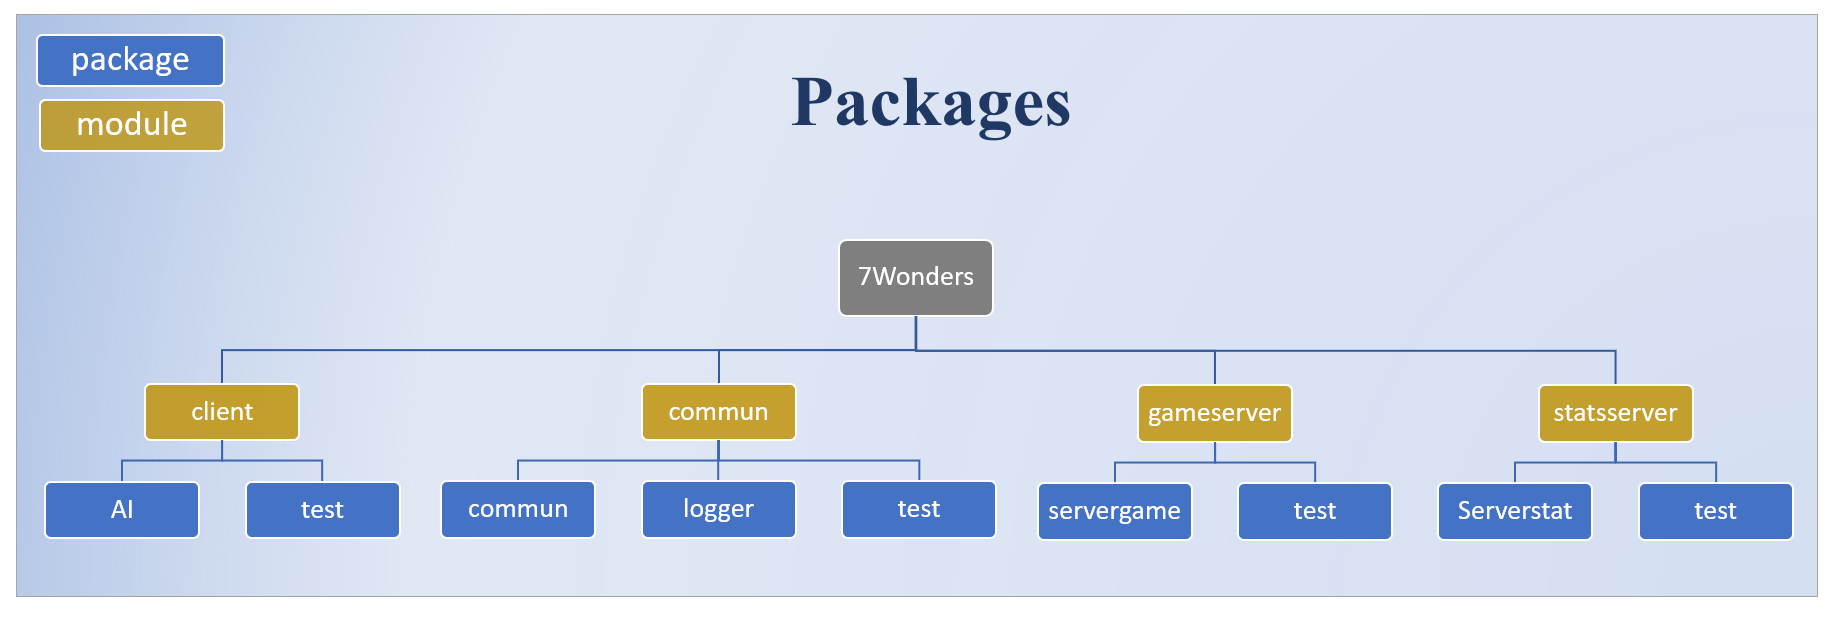
\includegraphics[scale=0.205]{Paquetages.png}
			\caption{Organisation générale des Packages}
		\end{center}
		\end{figure}

	\subsection{Hiérarchie d’héritages }
		\subsubsection{A.\hspace*{0.5cm}Classe abstraite :}
		\paragraph{}
 		\textbf{Dans le module « client » :}
 	\begin{itemize}
 	\item[•]\textbf{« AI » : }une classe abstraite qui implémente l’interface «RequestToPlayer» et qui est héritée par les classes «FirstAI», «SecondAI» et «RandomAI». Elle représente un modèle d’intelligence artificielle (IA).
 	\end{itemize}
 
		\begin{figure}[H]
		\begin{center}
			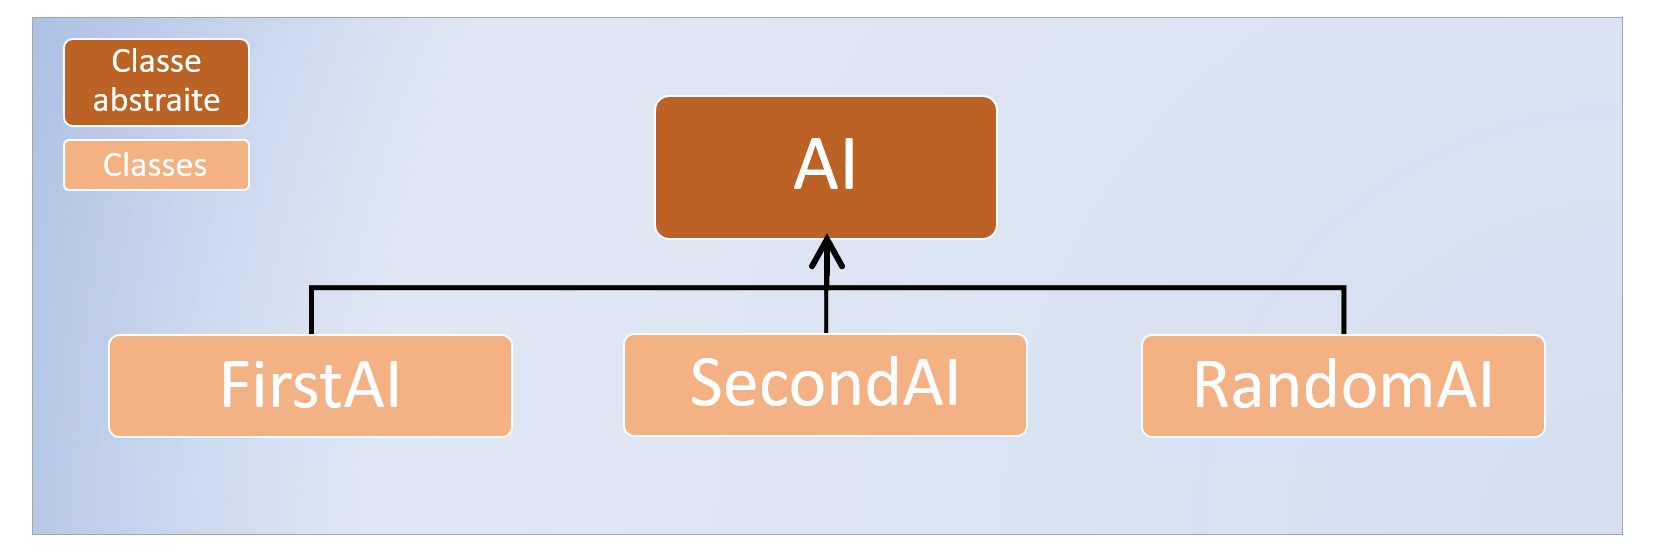
\includegraphics[scale=0.23]{ai.png}
			\caption{Héritages: AI}
		\end{center}
		\end{figure}
	
	\textbf{Dans le module « commun » :}
 	\begin{itemize}
	 	\item[•]\textbf{« AbstractAction » :} une classe abstraite héritée par les classes «BuildAction», «BuildStepAction», «DiscardAction» et «TradeAction». Elle représente un modèle de choix d’action que va effectuer une IA à chaque tour.
	 \end{itemize}  
	     
	 	\begin{figure}[H]
      	\begin{center}
			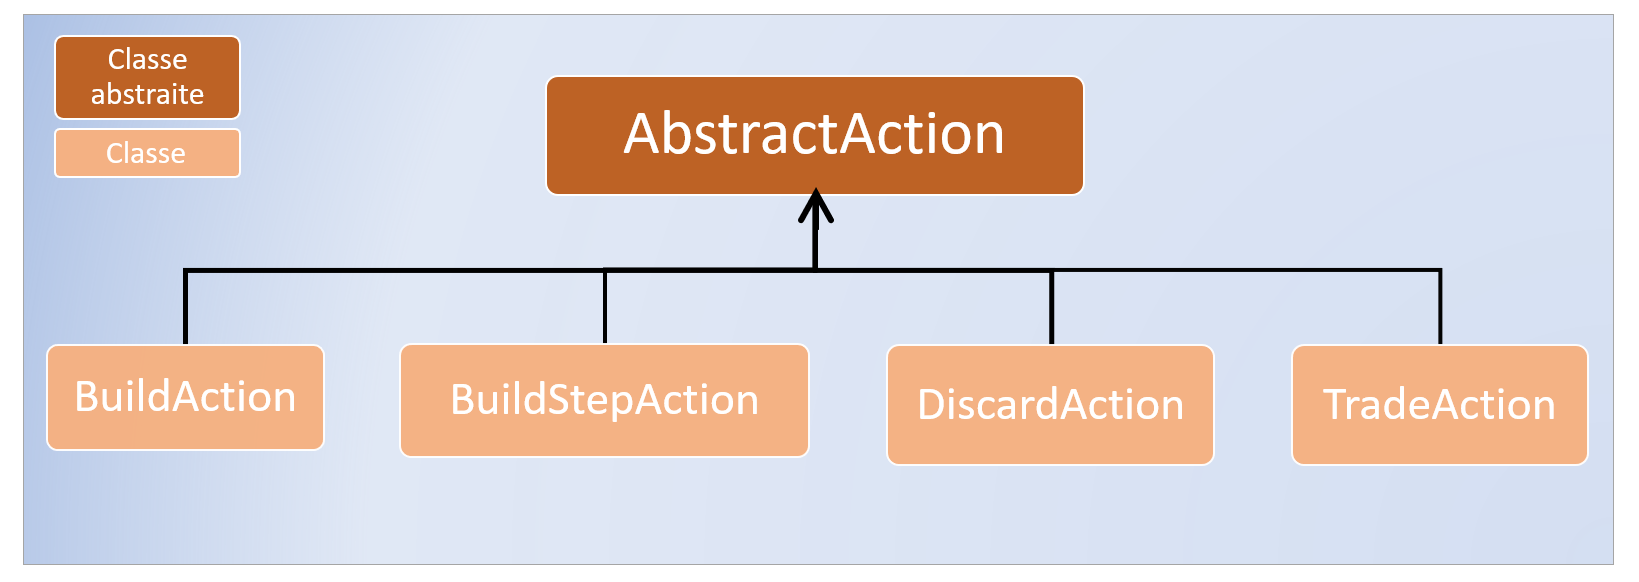
\includegraphics[scale=0.23]{action.png}
			\caption{Héritages: Action}
		\end{center}
		\end{figure}
	
	
 	\begin{itemize}
	 	\item[•]\textbf{« StatBase »:} une classe abstraite héritée par la classe «StatIntegerBase» qui elle-même sera héritée par toutes les classes de statistiques à base d’entiers. Elle représente un modèle de statistiques. 
	 	
    \end{itemize} 
		\begin{figure}[H]
      	\begin{center}
			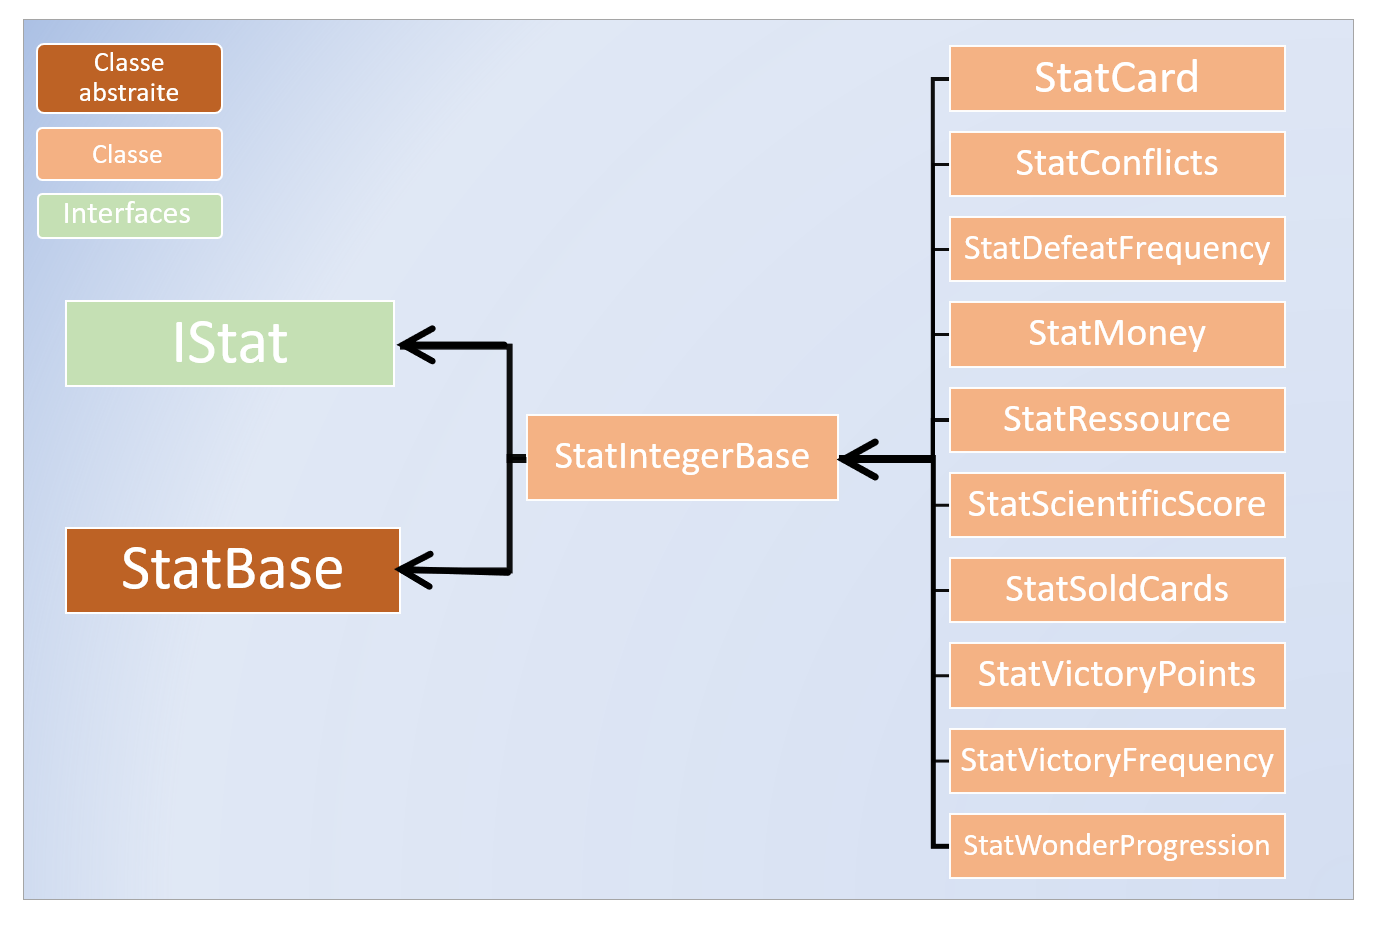
\includegraphics[scale=0.24]{stat.png}
			\caption{Héritages: Statistiques}
		\end{center}
		\end{figure}
	
		\subsubsection{B.\hspace*{0.5cm}Interfaces  :}
 		\paragraph{}
\textbf{Dans le module « commun » :}
 	\begin{itemize}
 	\item[•]\textbf{« ICost » :} une interface implémentée par toutes les classes «Cost», elle exige un modèle de coût (coût des cartes ou des étapes des merveilles) que celles-ci doivent implémenter. 
 	\item[•]\textbf{« IEffect » :} une interface implémentée par toutes les classes «Effect», elle exige un modèle d’effet ou gains (gains des différentes cartes et étapes des merveilles ainsi que les effets des guildes) que celles-ci doivent implémenter.
 	\item[•]\textbf{« PlayerRequestGame » :} une interface implémentée par la classe «PlayerController» dans le module « commun » et utilisée par la classe abstraite «AI» du module client pour permettre aux intelligences artificielles d’accéder à toutes les informations liées au joueur et à ses voisins.
 	\item[•]\textbf{« RequestToPlayer » :} une interface implémenter par la classe abstraite «AI» du module « client », elle permet donc d’exiger un modèle de tous les choix que devra faire les intelligences artificielles.
 	\item[•]\textbf{« IStat » :} une interface implémenter par la classe «StatIntegerBase», elle représente l’addition des statistiques. \\
 	\end{itemize}

\textbf{Dans le module « gameserver » :}
 	\begin{itemize}
 	\item[•]\textbf{« PlayerManager » :} une interface implémentée par la classe « PlayerManagerImpl », elle exige un modèle de direction de l’objet «player» durant la partie. Par exemple :\\
- \textit{Au début de la partie :} assigner le plateau et les voisins au joueur.\\
- \textit{Au début d’un tour :} assigner une main au joueur.\\
- \textit{Durant le tour :} demander à l’IA de faire un choix puis l’exécute.

 	\item[•]\textbf{« PlayerView » : } une interface implémentée par la classe «PlayerManagerImpl», elle permet au joueur d’avoir une vue globale du jeu, donc de voir ses voisins ainsi que l’ensemble des joueurs. \\
\end{itemize}

\textbf{Dans le module « statserver » :}
 	\begin{itemize}
 	\item[•]\textbf{« IDealer » :} une interface implémentée par la classe abstraite «DealerBase», ainsi elle exige que toutes les classes«Dealer» possèdent une méthode pour traiter les données et permettre de calculer les statistiques.
 	
 	\end{itemize}

	\subsection{Répartition des responsabilités et interaction entre les classes }
  		\subsubsection{A.\hspace*{0.5cm}Le Module client :}
 		\paragraph{}
 
Dans ce module, nous pouvons trouver trois intelligences artificielles (IAs) différentes.
Ces trois IAs utilisent toutes une classe abstraite « AI », qui représente les diverses fonctionnalités d’une intelligence artificielle.
Parmi les trois IA, chacune d’elle possède une stratégie unique.

\begin{flushleft}
 \textbf{- « RandomAI » : }Fait des choix aléatoires.\\
\textbf{- « FirstAI » :} Fait des choix par priorité (La priorité 1 (P1) étant la plus haute et la priorité 4 (P4) la plus basse) :
\begin{itemize}
\item[-]P1 : Points de victoire
\item[-]P2 : Matières premières
\item[-]P3 : Puissance militaires
\item[-]P4 : Défausse de cartes
\end{itemize}

\textbf{- « SecondAI » :} Fait des choix par priorité mais à chaque changement d’Âge, les priorités changent.
\begin{itemize}
\item[•] \textbf{Âge 1 :} 
    \begin{itemize}
     \item[-]P1 : Matières premières,
     \item[-]P2 : Bâtiments commerciaux
     \item[-]P3 : Produits manufacturés.
    \end{itemize}
\item[•] \textbf{Âge 2 :} 
   \begin{itemize}
     \item[-]P1 : Puissance militaire
	 \item[-]P2 : Construire une étape de merveille
	 \item[-]P3 : Points de victoire
\end{itemize}
\item[•] \textbf{Âge 3 : }
    \begin{itemize}
     \item[-]P1 : Points de victoire
     \item[-]P2 : Guilde
     \item[-]P3 : Bâtiments scientifiques
    \end{itemize}	
\end{itemize}

 \end{flushleft} 
    \subsubsection{B.\hspace*{0.5cm}Le Module commun :}
 	\paragraph{}

Dans ce module nous pouvons retrouver : 
\begin{flushleft}
- Le package « action » contient les classes qui correspondent aux actions qu’un joueur peut faire. 
\begin{itemize}
\item[•]
Les actions «BuildAction», «BuildStepAction», «DiscardAction» et «TradeAction», permettent respectivement de gérer la construction des bâtiments, construire une étape de merveille, défausser une carte et faire des échanges avec les autres joueurs. Elles sont toutes basées sur la classe abstraite «AbstractAction». \newline
\end{itemize}

- Le package « card » contient la représentation d’une carte (classe «Card») et d’un deck (classe «Deck»), qui est une liste de cartes. Chaque carte possède un type, représenté par l’enum «CardType».
\newline

- Le package « communication » envoie les statistiques du jeu au serveur. Il contient les classes «CommunicationMessages» (représente la communication entre le jeu et le serveur), «JsonUtils» (sert à désérialiser et sérialiser les paquets reçus par le serveur, «StatsObjects» (ensemble des statistiques envoyées au serveur). Il contient aussi un sous-package «statsobjects» permettant de calculer les différentes statistiques dans le jeu (exemple : la classe «StatConflicts» permet de faire des statistiques sur les conflits militaires).
\newline

- Le package « cost » représente le prix des cartes en pièces (classe «CoinCost») ou bien en matériaux (classe «MaterialCost»). La classe «MaterialCost» utilise deux autres classes : «MaterialCostSolver» qui permet d’obtenir les combinaisons possibles et valides d’acheter chez le joueur voisin et «MaterialCostArray» qui représente le prix des matériaux.
\newline

- Le package « effect » représente tous les effets que l’on peut retrouver sur les cartes du jeu. 
\newline

- Le package « material » représente les différents matériaux que l’on retrouve dans le jeu. Un matériau (classe «Material») a un nombre de ressources et un type (classe «MaterialType»). Ce package contient aussi la classe «ChoiceMaterial» qui permet de choisir entre plusieurs materiau.
\newline

- Le package « Player » correspond à la représentation d’un joueur par la classe Player.
\newline

- Le package « request » gère les requêtes données par les IA. Il permet de vérifier si l’action choisie par le joueur est valide grâce à la classe «RequestPlayerActionCheck».
\newline

- Le package « wonderboard » gère les points de conflits militaires par la classe «BattlePoint». Il contient aussi la représentation d’une merveille avec la classe «WonderBoard» ainsi que les étapes de merveilles qui correspondent à la classe «WonderStep».


\end{flushleft} 	  
		\subsubsection{C.\hspace*{0.5cm}Le Module « gameserver » :}
		\paragraph{}
 
Dans le module « gameserver » on retrouve :
\begin{flushleft}

-	Le package «card» contient les classes «CardFactory» et «CardManager». Elles permettent respectivement de : générer les decks de cartes suivant l’Âge et gérer les decks dans le jeu.
\newline

-	Le package «clientstats» contient la classe «SocketManager» qui permet de s’occuper de la gestion des paquets reçus par le serveur et renvoie les choix du joueur (IA) au serveur. 
\newline

-	Le package «engine» qui permet de gérer le déroulement d’une partie par le biais de la classe «GameEngine» et gérer l’effet Guilde des Scientifiques grâce à la classe «ScientistsGuildAction».
\newline

-	Le package «player» contient les interfaces «PlayerManager» et «PlayerView» et la classe «PlayerController» qui permet de contrôler les actions du joueur ainsi que la classe «PlayerManagerImpl» qui assigne les voisins, le plateau de jeu et crée la vue des joueurs . 
\newline

-	Le package «score» contient les classes «BattleScore» et «ScoreCalculator». Elles permettent respectivement le calcul de score des conflits militaires et le score total des joueurs.
\newline

-	La classe «WonderBoardFactory» qui permet la création des plateaux des merveilles du jeu avec la classe.
\newline

-	La classe «GameInitializer» qui permet d’initialiser une partie.
\newline

-	La classe « App» qui correspond au moteur de jeu. C’est ici qu’on lance les parties.

\end{flushleft}
		\subsubsection{D.\hspace*{0.5cm}Le Module « statsserver » :}
		\paragraph{} 
Ce module correspond au serveur de statistiques. Dans ce module, on peut retrouver :
\\
\begin{flushleft}
-	La classe « FileManager » qui permet la gestion d’un fichier pour les statistiques.
\newline

-	Le package « listerners » : contient les classes « StatsListener » et « FinishListener » qui permettent respectivement d’additionner les statistiques et mettre fin aux additions de statistiques.
\newline

-	Le package « stats » qui contient la classe « StatsObjectOrchestrer ». Cette classe permet d’afficher les statistiques sur la console et d’enregistrer celles-ci sous format CSV.
\newline
Cette classe utilise les classes contenues dans le package «dealers». Ces classes permettent de traiter les données et les renvoyer sous forme de listes de chaînes de caractères. 
\newline

-	La classe « Server » qui est une représentation du serveur.
\newline

-	La classe « App » qui permet de lancer le serveur.

\end{flushleft}

  \end{multicols} 
     
\newpage    
\setcounter{subsection}{0}      
\section*{Étude des patrons de conception}    
\addcontentsline{toc}{section}{Étude des patrons de conception} 
\begin{multicols}{2} 
      \paragraph{}     
      Les patrons de conception sont des solutions génériques pour des problèmes de conceptions logiciel. L’utilisation de ces derniers ont permis à travers notre projet de diminuer le couplage et de renforcer la cohésion entre classes/modules.
	\subsection{Patrons utilisés et justifications}
		\subsubsection{A.\hspace*{0.5cm}Patron Singleton}
 		\paragraph{}
      		Le patron Singleton permet l’utilisation d’une seule instance d’un objet, ce qui évite sa ré-instanciation. Cela a été utilisé avec les classes «GameLogger», qui permet d'avoir les informations en temps réel, et «StatModule», pour «StatModule» cela révèle l’utilisation d’un unique objet représentant les statistiques pour éviter son dispersement lourd dans des fonctions à besoin statistiques.
      		
		\subsubsection{B.\hspace*{0.5cm}Patron Factory}
		\paragraph{}
      		Le patron Factory nous a permis la génération des cartes en fonction du nombre de joueurs et des plateaux de merveille avec face aléatoire.   
			
		\subsubsection{C.\hspace*{0.5cm}Patron Template}
		\paragraph{}
Le patron Template a été utilisé sur la gestion des données statistiques, en effet même si la majorité des statistiques sont représentées des entiers, une crainte a été posée sur le possible changement de représentation de certaines statistiques (progression de la merveille, ...) et même l’ajout de statistiques avec une différente représentation. Donc l’ajout de statistiques et la conversion de celles-ci sont des patrons Template.

		\subsubsection{D.\hspace*{0.5cm}Patron Strategy}
		\paragraph{}
      		Le patron Strategy a été utilisé notamment sur les intelligences artificielles (IAs), en effet cela nous permet de gérer plus aisément leurs stratégies et leur interaction avec le jeu.
Ce patron a aussi été utilisé sur les coûts et sur les effets. On peut manipuler les coûts et les effets en passant par une même interface, ce qui permet la manipulation de ces fonctionnalités plus simple.

		\subsubsection{E.\hspace*{0.5cm}Patron Proxy}
		\paragraph{}
Le patron Proxy a été utilisé pour gérer les requêtes données par les IAs, notre proxy a fait office de vérifieur de données afin que les IAs ne puissent pas envoyer de données faussées ou tenter de tricher.

		\subsubsection{F.\hspace*{0.5cm}Patron Command}
		\paragraph{}

Ce patron définit la relation IA - jeu, l’IA passe par un patron Proxy pour effectuer une Action (il y a plusieurs actions possibles), et selon l’action et ses paramètres, nous modifions l’instance du jeu.
		\subsection{Patrons non retenus et justifications}
			\subsubsection{A.\hspace*{0.5cm}Patrons Observer et State}
      		\paragraph{}
      		Notre jeu fonctionne de façon séquentielle, il donne l’illusion au joueur (IA) qu’il se déroule de façon asynchrone, par conséquent il n'y a pas besoin de vérifier si un état change, puisque de façon séquentiel nous traitons les informations une à une, donc nous savons ce qu’il se passe étape par étape.

			\subsubsection{B.\hspace*{0.5cm}Patron Façade}
      		\paragraph{}
      		Nous pensons que notre code est assez bien découpé pour ne pas avoir à utiliser ce patron de conception, nous n’avons pas de sous-système assez complexe qui requiert ce patron.

\end{multicols}
\newpage


\setcounter{subsection}{0} 
\section*{Analyse de l'évolution métrique}  
\addcontentsline{toc}{section}{Analyse de l'évolution métrique}
\begin{multicols}{2} 

\paragraph{}
Dans cette partie nous allons voir itération par itération l’évolution des métriques de SonarQ et expliquer les éventuels changements entre celles-ci.
	\subsection{Itération 1}
	\paragraph{}
		\begin{figure}[H]
      	\begin{center}
			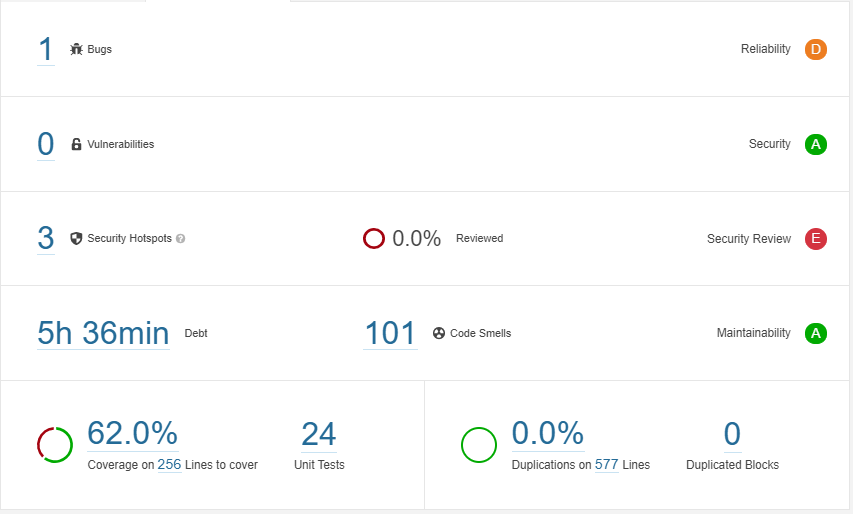
\includegraphics[scale=0.3]{1.png}
			\caption{SonarQ: Itération 1}
		\end{center}
		\end{figure}
	
L’itération 1 démarre avec deux classes non testées : «GameEngine» et «PlayerController» ce qui explique un coverage moyen. 
Les Security Hotspots sont dûs au new Random() de même pour le bug préconisant d’utiliser le même random et non d’en recréer un.
La dette technique est majoritairement augmentée par une classe inutile (commun.java) et des méthodes de test en public.  

	\subsection{Itération 2}
	\paragraph{}
        \begin{figure}[H]
      	\begin{center}
			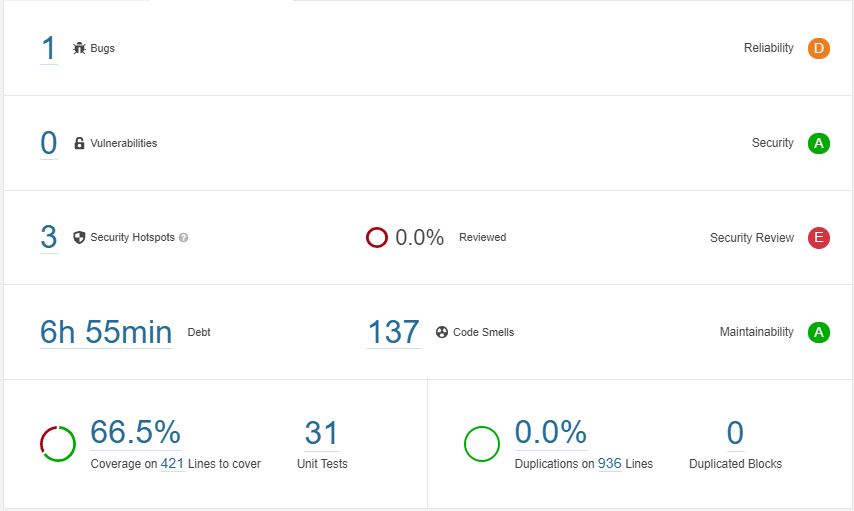
\includegraphics[scale=0.3]{2.png}
			\caption{SonarQ: Itération 2}
		\end{center}
		\end{figure}
L’itération 2 n’a aucune évolution majeure des métriques, les tests de «GameEngine» reste moyen (50\% testé). 
  	\subsection{Itération 3}
	\paragraph{}
        \begin{figure}[H]
      	\begin{center}
			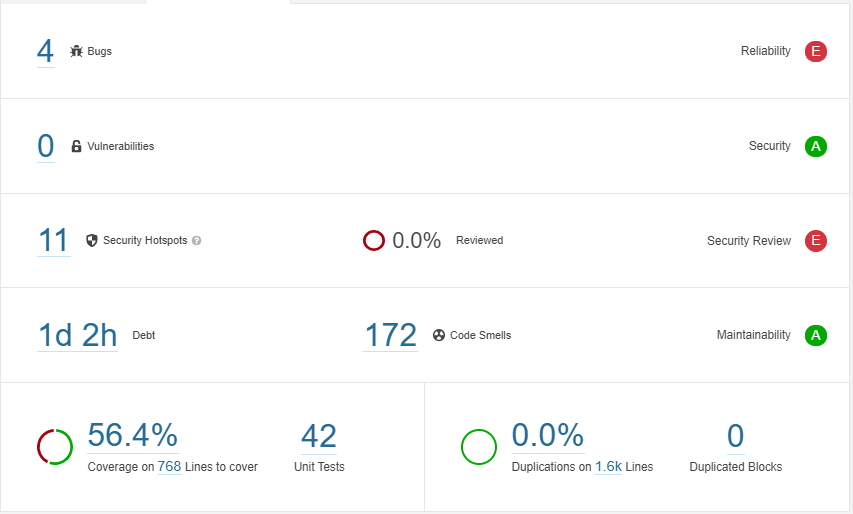
\includegraphics[scale=0.3]{3.png}
			\caption{SonarQ: Itération 3}
		\end{center}
		\end{figure}
L’itération 3 subit une baisse de toutes les métriques de SonarQ, les Security Hotspots sont dûs à des printStackTrace hors du logger. Les bugs quant à eux, à l’oublie de close() lors de la lecture de fichier.
La dette augmente fortement à cause du renvoie d’ArrayList par certaines fonctions et non l’interface «List». Également à cause des méthodes par défaut dans les interfaces.
	\subsection{Itération 4}
	\paragraph{}
        \begin{figure}[H]
      	\begin{center}
			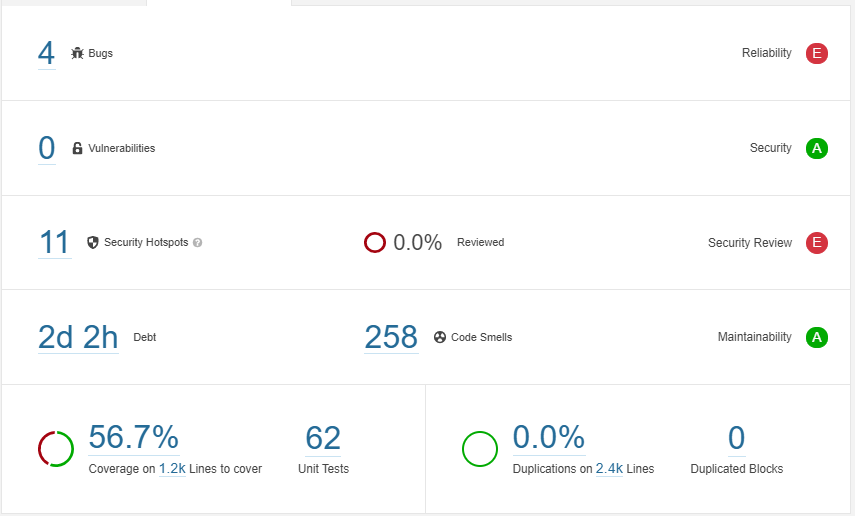
\includegraphics[scale=0.3]{4.png}
			\caption{SonarQ: Itération 4}
		\end{center}
		\end{figure}

L’itération 4 double presque la dette précédente. Cela se produit pour les mêmes raisons que les itérations précédentes, mais le code augmentant, le nombre de code smell augmente également.
  		\subsection{Itération 5}
      	\paragraph{}
        \begin{figure}[H]
      	\begin{center}
			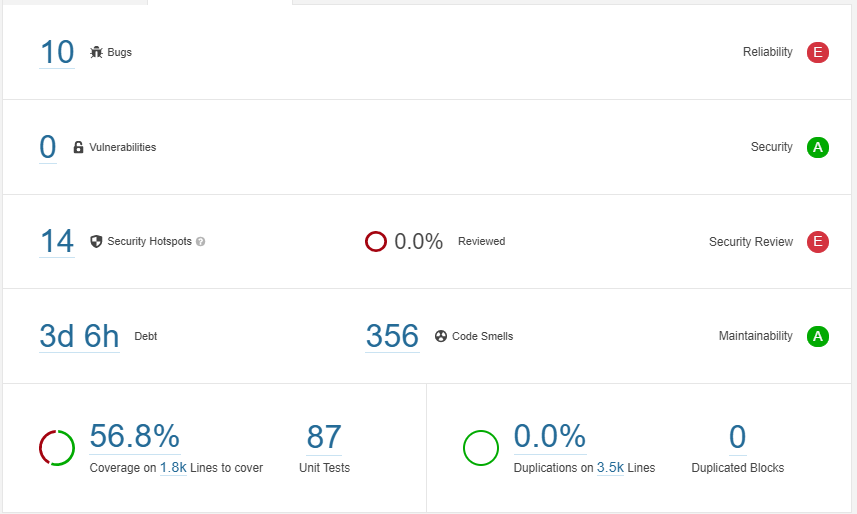
\includegraphics[scale=0.3]{5.png}
			\caption{SonarQ: Itération 5}
		\end{center}
		\end{figure}
L’itération 5 voit son nombre de bugs augmenté à cause d’objets potentiellements null (surtout dans la partie des statistiques). Les trois Security Hotspots ajoutés sont dûs au même raison ceux dit plus haut concernant les random().
La dette augmente d’un jour surtout à cause d’une fusion des classes entre «playerController» et les différentes actions (3h de dette à lui seul) et de nombreux switch case dans le code. 

  		\subsection{Itération 6}
      	\paragraph{}
        \begin{figure}[H]
      	\begin{center}
			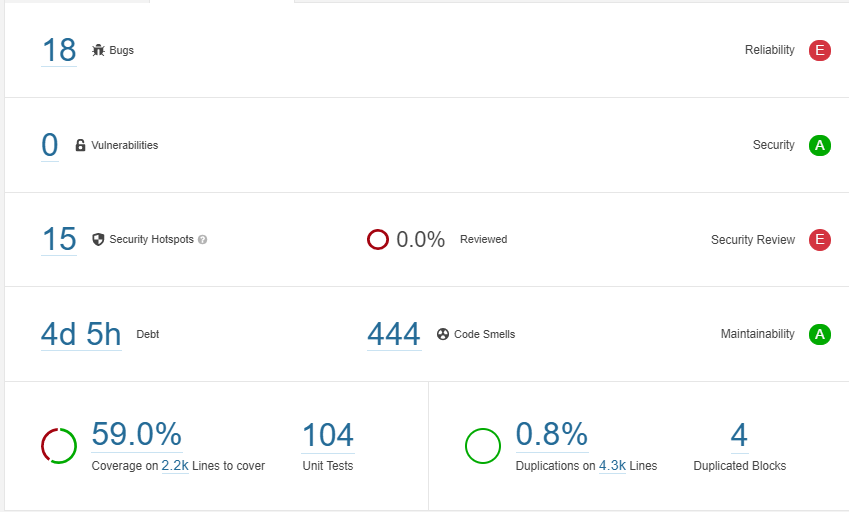
\includegraphics[scale=0.3]{6.png}
			\caption{SonarQ: Itération 6}
		\end{center}
		\end{figure}
L’itération 6 augmente de 8 le nombre de nouveaux bugs, un d’entre eux vient d’une boucle for qui ne s’arrête jamais (i = 4, i > 3, i++), et le reste de assertNotEquals entre deux types d’objet différent. La dette augmente encore d’une journée, «CardFactory» l’augmentant de 4h à cause de nombreuses string écrites en dur dans le code au lieu d’utiliser des constantes.

  		\subsection{Itération 7}
      	\paragraph{}
        \begin{figure}[H]
      	\begin{center}
			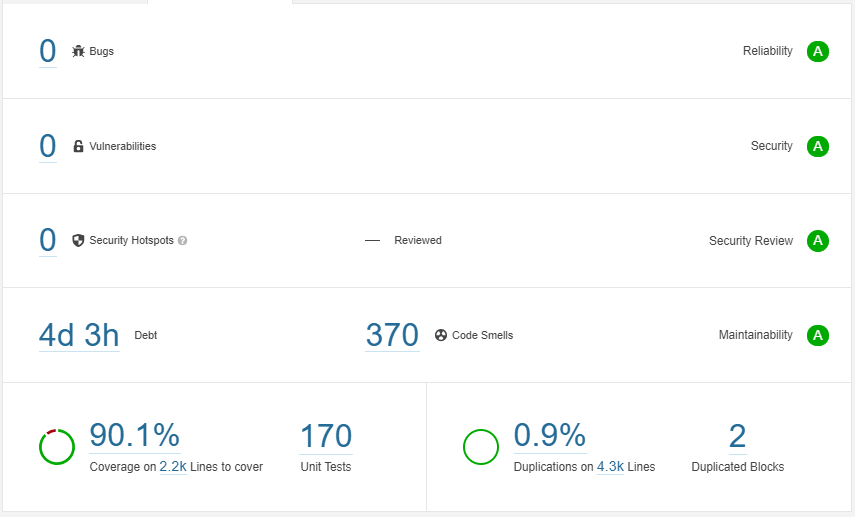
\includegraphics[scale=0.3]{7.png}
			\caption{SonarQ: Itération 7}
		\end{center}
		\end{figure}
Sur la 7ème et dernière itération, un effort a été effectué afin de corriger tous les bugs et problèmes de sécurité cités plus haut. De même, le coverage s’est nettement amélioré grâce aux tests de toutes les classes non triviales. La limite est atteinte à 90\% car de nombreuse classes composées de getters et setter ne sont alors pas testées.
\newline

Tout au long des itération un coverage de plus de 50\% à essayer d’être maintenu, ainsi qu’une bonne appréciation pour la maintenabilité et duplication du code. 
  


\section*{Conclusion}  
\addcontentsline{toc}{section}{Conclusion}  
	\paragraph{}
	Pour conclure, ce projet nous a permis de nous remettre à niveau avec tous nos nouveaux camarades. Malgré quelques légers retards notre projet est fini dans le temps imparti, il a fallu faire preuve d’ingéniosité et de créativité pour respecter les délais ainsi que d’implémenter correctement nos fonctionnalités tout en respectant nos contraintes technologiques.
\newline
En perspective, nous aurions voulu améliorer notre hygiène/nos pratiques de programmation en ce qui concerne le couvrage de nos tests mais aussi de la pertinence de nos \textit{commits}, ainsi nous aurions voulu séparer complètement les joueurs du jeu, et de sauvegarder dans une base de données nos statistiques.

\end{multicols}
\end{document}